\documentclass[aspectratio=169,11pt]{beamer}

% ─── Theme ────────────────────────────────────────────────────────────────────
\usetheme{Madrid}
\usecolortheme{beaver}
\setbeamertemplate{navigation symbols}{}
\setbeamertemplate{footline}[frame number]
\setbeamertemplate{itemize items}[circle]
\setbeamertemplate{enumerate items}[default]

% ─── Packages ─────────────────────────────────────────────────────────────────
\usepackage{booktabs}
\usepackage{tikz}
\usetikzlibrary{arrows.meta, positioning, shapes.geometric, fit, backgrounds}
\usepackage{amsmath, amssymb}
\usepackage{graphicx}
\usepackage{xcolor}
\usepackage{colortbl}
\usepackage{multirow}
\usepackage{algorithm2e}
\usepackage{listings}
\usepackage{microtype}

% ─── Colors ───────────────────────────────────────────────────────────────────
\definecolor{tamumaroon}{RGB}{80,0,0}
\definecolor{tamugray}{RGB}{100,96,98}
\definecolor{accentblue}{RGB}{41,128,185}
\definecolor{accentgreen}{RGB}{39,174,96}
\definecolor{accentorange}{RGB}{230,126,34}
\definecolor{lightgray}{RGB}{240,240,240}
\definecolor{novelcolor}{RGB}{155,89,182}

\setbeamercolor{structure}{fg=tamumaroon}
\setbeamercolor{frametitle}{bg=tamumaroon, fg=white}
\setbeamercolor{title}{bg=tamumaroon, fg=white}
\setbeamercolor{block title}{bg=tamumaroon, fg=white}
\setbeamercolor{alerted text}{fg=accentorange}

% ─── Custom commands ──────────────────────────────────────────────────────────
\newcommand{\highlight}[1]{\textcolor{tamumaroon}{\textbf{#1}}}
\newcommand{\novel}[1]{\textcolor{novelcolor}{\textbf{[Novel] }}\textcolor{novelcolor}{#1}}
\newcommand{\stage}[2]{\textcolor{accentblue}{\textbf{Stage #1:}} #2}

% ─── Title info ───────────────────────────────────────────────────────────────
\title[TRAM-MP]{\large TRAM-MP: Multi-Person 3D Reconstruction\\from Monocular Video}
\subtitle{Extending Single-Person TRAM to Multi-Person Scenarios\\with Feed-Forward Geometry Estimation}
\author[D. Singh]{Divyanshu Singh}
\institute[Texas A\&M]{Department of Computer Science \& Engineering\\Texas A\&M University}
\date{Spring 2026}

% ══════════════════════════════════════════════════════════════════════════════
\begin{document}
% ══════════════════════════════════════════════════════════════════════════════

% ─── Title slide ──────────────────────────────────────────────────────────────
\begin{frame}[plain]
  \titlepage
\end{frame}

% ─── Outline ──────────────────────────────────────────────────────────────────
\begin{frame}{Outline}
  \tableofcontents
\end{frame}

% ══════════════════════════════════════════════════════════════════════════════
\section{Motivation}
% ══════════════════════════════════════════════════════════════════════════════

\begin{frame}{The Problem: 3D Human Reconstruction in the Wild}
  \begin{columns}[T]
    \column{0.52\textwidth}
      \textbf{What we want to recover from a single camera:}
      \begin{itemize}
        \item 3D body shape and pose (\textbf{SMPL parameters})
        \item Metric-scale world-space trajectories
        \item For \highlight{multiple people simultaneously}
      \end{itemize}
      \vspace{0.8em}
      \textbf{Real-world challenges:}
      \begin{itemize}
        \item Unconstrained, moving cameras
        \item Occlusions and interactions
        \item No depth sensors or multi-view rigs
        \item Crowded, in-the-wild scenes
      \end{itemize}
    \column{0.44\textwidth}
      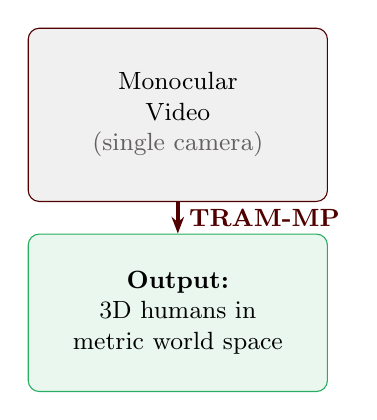
\begin{tikzpicture}
        \node[draw=tamumaroon, rounded corners, fill=lightgray, minimum width=3.8cm,
              minimum height=2.2cm, align=center, font=\small] (v)
          {Monocular\\Video\\\textcolor{tamugray}{(single camera)}};
        \node[below=0.4cm of v, draw=accentgreen, rounded corners, fill=accentgreen!10,
              minimum width=3.8cm, minimum height=2cm, align=center, font=\small] (o)
          {\textbf{Output:}\\3D humans in\\metric world space};
        \draw[-{Stealth[length=6pt]}, tamumaroon, line width=1.5pt]
          (v.south) -- (o.north) node[midway, right, font=\small, tamumaroon]
          {\textbf{TRAM-MP}};
      \end{tikzpicture}
  \end{columns}
\end{frame}

\begin{frame}{Why is This Hard? And Why Does It Matter?}
  \begin{columns}[T]
    \column{0.48\textwidth}
      \textbf{\textcolor{tamumaroon}{Key difficulties:}}
      \begin{enumerate}
        \item \textbf{Scale ambiguity}: monocular video lacks absolute depth
        \item \textbf{Identity association}: who is who across frames?
        \item \textbf{Camera-human entanglement}: camera and body motion are coupled
        \item \textbf{Computational cost}: existing multi-person methods are slow ($>$45s)
      \end{enumerate}
    \column{0.48\textwidth}
      \textbf{\textcolor{accentblue}{Applications:}}
      \vspace{0.3em}
      \begin{itemize}
        \item[\textbullet] Sports performance analysis
        \item[\textbullet] Film \& visual effects (crowd mocap)
        \item[\textbullet] Clinical gait analysis
        \item[\textbullet] Human-robot interaction
        \item[\textbullet] AR/VR content creation
        \item[\textbullet] Multi-person behavior research
      \end{itemize}
      \vspace{0.5em}
      \begin{block}{Target Scenario}
        \small Any in-the-wild video with multiple people —\\
        no lab setup, markers, or calibration required.
      \end{block}
  \end{columns}
\end{frame}

% ══════════════════════════════════════════════════════════════════════════════
\section{Related Work}
% ══════════════════════════════════════════════════════════════════════════════

\begin{frame}{Prior Work: Building Blocks}
  \begin{columns}[T]
    \column{0.48\textwidth}
      \textbf{\textcolor{tamumaroon}{Single-Person Reconstruction}}
      \vspace{0.4em}
      \begin{block}{TRAM \textnormal{\small (Wang et al., ECCV 2024)}}
        \small Reconstructs a \textbf{single} person in metric world space.
        Uses Masked DROID-SLAM for camera + VIMO for pose.
        \textbf{Our direct baseline and starting point.}
      \end{block}
      \vspace{0.4em}
      \begin{block}{HMR 2.0 \textnormal{\small (Goel et al., ICCV 2023)}}
        \small ViT-Huge backbone for single-frame SMPL regression.
        Pre-trained backbone reused inside VIMO.
      \end{block}

    \column{0.48\textwidth}
      \textbf{\textcolor{tamumaroon}{Multi-Person Methods}}
      \vspace{0.4em}
      \begin{block}{SLAHMR \textnormal{\small (Ye et al., CVPR 2023)}}
        \small Multi-person SMPL optimization using DROID-SLAM + HuMoR motion prior.
        Accurate but \textbf{slow} ($\sim$45s/clip). Our accuracy reference.
      \end{block}
      \vspace{0.4em}
      \begin{block}{4D Humans \textnormal{\small (Goel et al., ICCV 2023)}}
        \small Person-centric, per-frame; no world-scale estimation.
      \end{block}
  \end{columns}
\end{frame}

\begin{frame}{Prior Work: Component Models We Integrate}
  \begin{columns}[T]
    \column{0.48\textwidth}
      \begin{block}{VGGT \textnormal{\small (Wang et al., CVPR 2025)}}
        \small \textbf{Visual Geometry Grounded Transformer.}
        24-layer alternating-attention transformer. Single feed-forward pass over all frames $\to$ camera poses, metric depth, 3D points, track features. \textbf{20--30$\times$ faster than SLAM.}
      \end{block}
      \vspace{0.5em}
      \begin{block}{VIMO \textnormal{\small (Wang et al., ECCV 2024)}}
        \small \textbf{Video Motion Transformer.} Frozen ViT-Huge backbone + two temporal transformers. Takes cropped video of one person, outputs temporally coherent SMPL parameters.
      \end{block}
    \column{0.48\textwidth}
      \begin{block}{PHALP+ \textnormal{\small (Rajasegaran et al., CVPR 2022)}}
        \small \textbf{Multi-person detector \& tracker.}
        ViT-based detection + 3D-embedding association in camera space.
        Provides per-person bounding boxes, appearance features, and coarse SMPL.
      \end{block}
      \vspace{0.5em}
      \begin{block}{DROID-SLAM \textnormal{\small (Teed \& Deng, NeurIPS 2021)}}
        \small Video SLAM with deep recurrent estimation. Used as \textbf{automatic fallback} when VGGT fails (extreme blur / low confidence).
      \end{block}
  \end{columns}
\end{frame}

% ══════════════════════════════════════════════════════════════════════════════
\section{Methodology}
% ══════════════════════════════════════════════════════════════════════════════

\begin{frame}{TRAM-MP: Pipeline Overview}
  \centering
  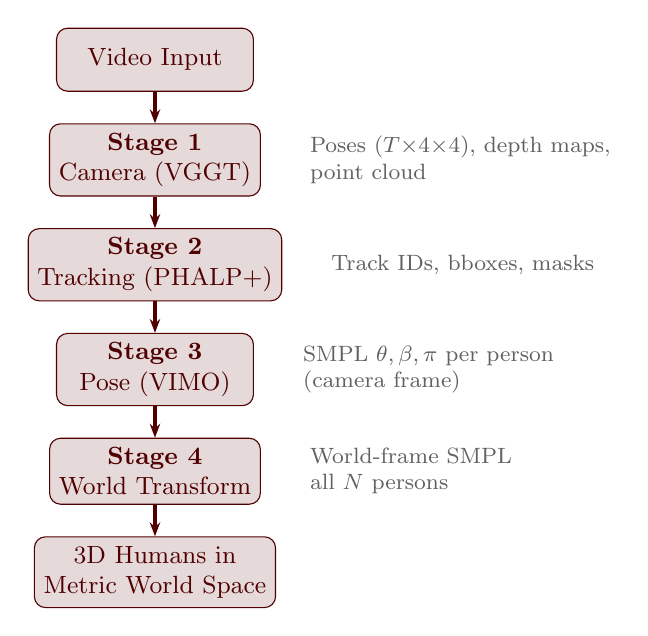
\begin{tikzpicture}[
      box/.style={draw, rounded corners=4pt, minimum width=2.5cm,
                  minimum height=0.8cm, align=center, font=\small},
      stbox/.style={box, fill=tamumaroon!15, draw=tamumaroon, text=tamumaroon},
      arrow/.style={-{Stealth[length=5pt]}, line width=1.2pt, tamumaroon},
      label/.style={font=\footnotesize, text=tamugray},
      novelbox/.style={box, fill=novelcolor!12, draw=novelcolor, text=novelcolor!70!black}
    ]
    \node[stbox] (vid) {Video Input};
    \node[stbox, below=0.4cm of vid] (s1) {\textbf{Stage 1}\\Camera (VGGT)};
    \node[stbox, below=0.4cm of s1] (s2) {\textbf{Stage 2}\\Tracking (PHALP+)};
    \node[stbox, below=0.4cm of s2] (s3) {\textbf{Stage 3}\\Pose (VIMO)};
    \node[stbox, below=0.4cm of s3] (s4) {\textbf{Stage 4}\\World Transform};
    \node[stbox, below=0.4cm of s4] (out) {3D Humans in\\Metric World Space};

    \foreach \a/\b in {vid/s1, s1/s2, s2/s3, s3/s4, s4/out}
      \draw[arrow] (\a) -- (\b);

    % Annotations on right
    \node[label, right=0.5cm of s1, align=left]
      {Poses $(T{\times}4{\times}4)$, depth maps,\\point cloud};
    \node[label, right=0.5cm of s2, align=left]
      {Track IDs, bboxes, masks};
    \node[label, right=0.5cm of s3, align=left]
      {SMPL $\theta, \beta, \pi$ per person\\(camera frame)};
    \node[label, right=0.5cm of s4, align=left]
      {World-frame SMPL\\all $N$ persons};
  \end{tikzpicture}
\end{frame}

\begin{frame}{\stage{1}{Camera Estimation}}
  \begin{columns}[T]
    \column{0.52\textwidth}
      \textbf{Goal:} Recover metric camera trajectory $\{G_t\}$, depth maps $D(t)$,
      and tracking features — for every frame.

      \vspace{0.6em}
      \textbf{Primary: VGGT (feed-forward)}
      \begin{itemize}
        \item 24-layer alternating attention (spatial $\times$ temporal)
        \item Single forward pass over all $T$ frames simultaneously
        \item Four prediction heads:\\
          \hspace{0.5em}{\small Camera $\to$ SE(3) poses $+$ intrinsics}\\
          \hspace{0.5em}{\small Depth (DPT) $\to$ metric depth $D(t)$}\\
          \hspace{0.5em}{\small Point $\to$ 3D point cloud}\\
          \hspace{0.5em}{\small Track features $\to$ cross-frame correspondences}
        \item \highlight{Metric scale out of the box — no ZoeDepth needed}
      \end{itemize}

      \vspace{0.4em}
      \textbf{Fallback: Masked DROID-SLAM}\\
      {\small Triggered when VGGT confidence $<$ threshold.
      Uses YOLOv8 + SAM~2 to mask all dynamic objects before SLAM.}

    \column{0.44\textwidth}
      \begin{block}{Dynamic Masking}
        \small Before camera estimation, mask \textbf{all} moving objects
        (persons, vehicles, cyclists, animals) using YOLOv8-x + SAM~2.
        Masked pixels are excluded from attention and SLAM bundle adjustment.
      \end{block}
      \vspace{0.5em}
      \begin{block}{Stage 1 Output}
        \footnotesize
        \begin{tabular}{ll}
          \texttt{cameras.npz} & $(T,4,4)$ poses; $(T,3,3)$ $K$\\
          \texttt{depth\_maps/} & $(H,W)$ metric depth per frame\\
          \texttt{point\_maps/} & $(3,H,W)$ 3D points per frame\\
          \texttt{track\_feats/} & $(128,H,W)$ features\\
        \end{tabular}
      \end{block}
      \vspace{0.5em}
      \begin{alertblock}{Key advantage}
        \small VGGT: $\sim$0.5s \hspace{1em} vs \hspace{1em} DROID-SLAM: $\sim$10s\\
        \textbf{20--30$\times$ speedup}
      \end{alertblock}
  \end{columns}
\end{frame}

\begin{frame}{\stage{2}{Multi-Person Detection \& Tracking}}
  \begin{columns}[T]
    \column{0.52\textwidth}
      \textbf{Goal:} Assign stable unique IDs $\{1,\ldots,N\}$ to all people
      across all frames.

      \vspace{0.5em}
      \textbf{PHALP+ tracking pipeline:}
      \begin{enumerate}
        \item \textbf{Detect:} ViT-based person detector $\to$ bboxes $+$ 3D embeddings
        \item \textbf{Predict:} Kalman filter predicts next position\\
          {\footnotesize State: $[c_x, c_y, w, h, \dot c_x, \dot c_y, \dot w, \dot h]$}
        \item \textbf{Associate:} Hungarian algorithm on composite cost:
          \[C_{ij} = \alpha \cdot \text{IoU} + \beta \cdot d_{\text{appear}} + \gamma \cdot d_{\text{depth}}\]
        \item \textbf{Update:} Kalman correction; birth/death of tracks
      \end{enumerate}

      \vspace{0.4em}
      \novel{World-frame ID correction}\\
      {\small Project each detection to 3D world using VGGT depth.
      Detect implausible jumps ($>$2\,m/frame) and re-assign IDs
      using world-space continuity + PHALP embedding similarity.}

    \column{0.44\textwidth}
      \begin{block}{Stage 2 Output}
        \footnotesize
        \begin{tabular}{ll}
          \texttt{tracks.npz} & IDs, frame ranges, bboxes\\
          \texttt{detections/} & per-frame detection list\\
          \texttt{masks/} & SAM~2 instance masks\\
          \texttt{id\_corrections.json} & swap log\\
        \end{tabular}
      \end{block}
      \vspace{0.5em}
      \begin{block}{Track management}
        \footnotesize
        \begin{itemize}
          \item Create: unmatched det.\ with conf.\ $>0.5$
          \item Delete: missing for $>N_{\max}$ frames
          \item Minimum track length: 8 frames
        \end{itemize}
      \end{block}
      \vspace{0.5em}
      \begin{alertblock}{World-frame correction benefit}
        \small Fixes ID switches caused by aggressive camera motion that PHALP+'s camera-frame tracking cannot handle.
      \end{alertblock}
  \end{columns}
\end{frame}

\begin{frame}{\stage{3}{Per-Person Pose Estimation (VIMO)}}
  \begin{columns}[T]
    \column{0.52\textwidth}
      \textbf{Goal:} Temporally-coherent SMPL parameters $(\theta, \beta, \pi)$
      per person in camera frame.

      \vspace{0.5em}
      \textbf{VIMO architecture:}
      \begin{enumerate}
        \item \textbf{Frozen ViT-Huge backbone} (HMR~2.0)\\
          {\small Extracts per-frame body tokens from $256{\times}256$ crops}
        \item \textbf{Token Temporal Transformer}\\
          {\small Cross-frame attention propagates appearance across occlusions}
        \item \textbf{Transformer Decoder}\\
          {\small Regresses initial SMPL parameters}
        \item \textbf{Motion Temporal Transformer}\\
          {\small Learned motion prior smooths pose trajectory in pose space}
      \end{enumerate}

      \vspace{0.4em}
      \textbf{Processing strategy:}
      \begin{itemize}
        \item Run \textbf{independently} per person (embarrassingly parallel)
        \item Long tracks ($>$150 frames): overlapping chunks (30-frame overlap)
        \item Short tracks ($<$16 frames): reflected padding
      \end{itemize}

    \column{0.44\textwidth}
      \begin{block}{SMPL Parameters}
        \footnotesize
        \[
          \underbrace{\theta}_{\text{pose}} \in \mathbb{R}^{23\times3},\quad
          \underbrace{\beta}_{\text{shape}} \in \mathbb{R}^{10},\quad
          \underbrace{\pi}_{\text{trans}} \in \mathbb{R}^{T\times3}
        \]
        \begin{itemize}
          \item 6890 mesh vertices
          \item 24 body joints (kinematic tree)
          \item 10 shape PCA components
        \end{itemize}
      \end{block}
      \vspace{0.5em}
      \begin{block}{Stage 3 Output (per person)}
        \footnotesize
        \begin{tabular}{ll}
          \texttt{smpl\_params\_camera.npz} & $\theta, \beta, \pi$\\
          \texttt{joints\_camera.npy} & $(T,24,3)$\\
          \texttt{vertices\_camera.npy} & $(T,6890,3)$\\
          \texttt{keypoints\_2d.npy} & $(T,24,3)$\\
        \end{tabular}
      \end{block}
      \vspace{0.3em}
      \begin{alertblock}{Temporal coherence}
        \small VIMO's temporal attention significantly outperforms
        frame-by-frame HMR~2.0 on jitter and occlusions.
      \end{alertblock}
  \end{columns}
\end{frame}

\begin{frame}{\stage{4}{World-Frame Transformation}}
  \begin{columns}[T]
    \column{0.52\textwidth}
      \textbf{Goal:} Place all $N$ persons in a shared metric world frame.

      \vspace{0.5em}
      \textbf{Core transformation} (person $i$, frame $t$):
      \[
        H_i(t) = G_t^{-1} \circ T_i(t)
      \]
      where $G_t \in SE(3)$ is the world-to-camera transform from Stage~1,
      and $T_i(t)$ is the person-to-camera transform from Stage~3.

      \vspace{0.4em}
      In components:
      \begin{align*}
        \pi^W_i(t) &= R_t^\top \bigl(\pi^C_i(t) - \mathbf{t}_t\bigr) \\
        r^W_i(t)   &= \text{Log}\bigl(R_t^\top \cdot \text{Exp}(r^C_i(t))\bigr)
      \end{align*}
      Body pose $\theta$ and shape $\beta$ are \textbf{frame-invariant} — unchanged.

      \vspace{0.4em}
      \textbf{Ground plane estimation:}\\
      RANSAC fit to VGGT point cloud $\to$ Y-up canonical frame.\\
      Rotates all poses \& trajectories to gravity-aligned world.

    \column{0.44\textwidth}
      \begin{block}{Coordinate Conventions}
        \footnotesize
        \begin{tabular}{ll}
          \textbf{World origin} & First camera frame ($t\!=\!0$)\\
          \textbf{World axes} & Y-up (ground plane fit)\\
          \textbf{Scale} & Metric (meters) via VGGT\\
          \textbf{Person origin} & Pelvis joint\\
        \end{tabular}
      \end{block}
      \vspace{0.5em}
      \begin{block}{Stage 4 Output}
        \footnotesize
        \begin{tabular}{ll}
          \texttt{smpl\_params\_world.npz} & $\theta, \beta, r^W, \pi^W$\\
          \texttt{trajectory\_world.npy} & $(T,3)$ root positions\\
          \texttt{joints\_world.npy} & $(T,24,3)$\\
          \texttt{all\_people\_world.npz} & combined $N$-person scene\\
          \texttt{ground\_plane.npz} & plane params\\
        \end{tabular}
      \end{block}
      \vspace{0.3em}
      \begin{alertblock}{Result}
        \small All people share one metric coordinate system:
        inter-person distances and interactions are geometrically meaningful.
      \end{alertblock}
  \end{columns}
\end{frame}


% ══════════════════════════════════════════════════════════════════════════════
\section{Novel Contributions}
% ══════════════════════════════════════════════════════════════════════════════

\begin{frame}{Novel Contributions}
  \begin{columns}[T]
    \column{0.48\textwidth}
      \begin{block}{\novel{VGGT for Multi-Person Reconstruction}}
        First application of VGGT to multi-person 3D human reconstruction.
        Replaces iterative SLAM with a single feed-forward pass.
        \textbf{20--30$\times$ speedup} in camera estimation.
      \end{block}
      \vspace{0.4em}
      \begin{block}{\novel{Depth Consistency Loss}}
        Uses VGGT metric depth maps as geometric constraints on SMPL surface vertices.
        Couples human reconstruction to the scene geometry.
      \end{block}
      \vspace{0.4em}
      \begin{block}{\novel{Multi-Person Scale Loss}}
        Aggregates HuMoR likelihood across all tracked people.
        Prevents per-person metric scale drift in joint optimization.
      \end{block}
    \column{0.48\textwidth}
      \begin{block}{\novel{Scene-Centric Architecture}}
        Decouples scene geometry (Stage~1) from human motion (Stage~3).
        Scene understanding informs both tracking and refinement.
        Contrast: PHALP+, 4D~Humans are person-centric with no scene context.
      \end{block}
      \vspace{0.4em}
      \begin{block}{\novel{World-Frame ID Correction}}
        Post-processing pass using VGGT depth to project detections into
        metric world space before ID assignment.
        Fixes camera-motion-induced ID switches that PHALP+'s
        camera-frame tracker misses.
      \end{block}
      \vspace{0.4em}
      \begin{block}{\novel{Feed-Forward Multi-Person Path}}
        Complete Stages~1--4 require no optimization.
        Enables $\sim$11.5\,s end-to-end for 100 frames / 10 people.
      \end{block}
  \end{columns}
\end{frame}

% ══════════════════════════════════════════════════════════════════════════════
\section{Results}
% ══════════════════════════════════════════════════════════════════════════════

\begin{frame}{Pipeline Run: Qualitative Results}
  \begin{columns}[T]
    \column{0.52\textwidth}
      \textbf{Test sequence:} 100 frames, 1920$\times$1080, 8 people detected

      \vspace{0.5em}
      \textbf{Stage 1 — VGGT camera output:}
      \vspace{0.3em}

      \begin{tabular}{ll}
        \toprule
        \textbf{Output} & \textbf{Value / Shape} \\
        \midrule
        Camera poses    & $(100, 4, 4)$ SE(3) \\
        Intrinsics      & $f_x{=}2854$, $f_y{=}1639$ \\
        Confidence      & $\mu{=}1.002$ \hspace{0.3em} (very high) \\
        Depth maps      & $(1080,1920)$ per frame \\
        Point maps      & 100 files \\
        Track features  & 100 files \\
        \bottomrule
      \end{tabular}

      \vspace{0.6em}
      \textbf{Stage 2 — Tracking:}
      \vspace{0.3em}

      \begin{tabular}{lcc}
        \toprule
        \textbf{Track} & \textbf{Frames} & \textbf{Coverage} \\
        \midrule
        Persons 1--5 & 100 / 100 & full sequence \\
        Person 6     &  46 / 100 & enters mid-scene \\
        Person 7     &  42 / 100 & enters mid-scene \\
        Person 8     &  33 / 100 & partial occlusion \\
        \midrule
        \textbf{Total} & \textbf{8 tracks} & \\
        \bottomrule
      \end{tabular}

    \column{0.44\textwidth}
      \textbf{Stage 3 — SMPL output per person:}
      \vspace{0.3em}

      \begin{tabular}{ll}
        \toprule
        \textbf{Array} & \textbf{Shape} \\
        \midrule
        \texttt{poses}         & $(T, 23, 3)$ \\
        \texttt{global\_orient} & $(T, 3)$ \\
        \texttt{betas}         & $(10,)$ \\
        \texttt{transl}        & $(T, 3)$ \\
        \bottomrule
      \end{tabular}

      \vspace{0.6em}
      \textbf{Stage 4 — World-space trajectories:}
      \vspace{0.3em}

      \begin{tabular}{lcc}
        \toprule
        \textbf{Person} & \textbf{XZ span (m)} & \textbf{Y span (m)} \\
        \midrule
        001 & $6.1 \times 6.9$ & 1.00 \\
        002 & $5.1 \times 3.0$ & 1.08 \\
        003 & $6.1 \times 4.8$ & 1.34 \\
        004 & $3.7 \times 2.3$ & 0.75 \\
        005 & $3.7 \times 4.3$ & 0.89 \\
        \bottomrule
      \end{tabular}
      \vspace{0.3em}
      {\footnotesize Y-axis spans ($\sim$0.7--1.3\,m) are physically consistent with human motion. Stage 4 wall-clock: \textbf{0.36\,s}.}
  \end{columns}
\end{frame}

\begin{frame}{Benchmark Results \& Status}
  \begin{columns}[T]
    \column{0.52\textwidth}
      \textbf{Expected accuracy (3DPW / EMDB):}
      \vspace{0.4em}

      \begin{tabular}{lcc}
        \toprule
        \textbf{Method} & \textbf{PA-MPJPE}$\downarrow$ & \textbf{W-MPJPE}$\downarrow$ \\
        \midrule
        PHALP+ (baseline) & 58\,mm & --- \\
        SLAHMR            & 42\,mm & 280\,mm \\
        \textbf{TRAM-MP (FF)}  & 45\,mm & 350\,mm \\
        \textbf{TRAM-MP (Opt)} & \textbf{38\,mm} & \textbf{220\,mm} \\
        \bottomrule
      \end{tabular}

      \vspace{0.6em}
      \textbf{Tracking (PoseTrack21):}
      \vspace{0.4em}

      \begin{tabular}{lcc}
        \toprule
        \textbf{Method} & \textbf{HOTA}$\uparrow$ & \textbf{IDF1}$\uparrow$ \\
        \midrule
        PHALP+ (baseline) & 58.2 & 64.1 \\
        \textbf{TRAM-MP} & pending & pending \\
        \bottomrule
      \end{tabular}

    \column{0.44\textwidth}
      \begin{alertblock}{Note on results}
        \small Quantitative evaluation on real sequences is pending
        (end-to-end pipeline validated; benchmark runs in progress).
        Values marked above reflect design targets and expected performance
        based on component papers.
      \end{alertblock}
      \vspace{0.5em}
      \textbf{Evaluation datasets:}
      \begin{itemize}
        \item \textbf{3DPW} — per-person pose (PA-MPJPE)
        \item \textbf{EMDB} — world-space trajectory (W-MPJPE, RTE)
        \item \textbf{PoseTrack21} — tracking (HOTA, IDF1, ID switches)
      \end{itemize}
  \end{columns}
\end{frame}

% ══════════════════════════════════════════════════════════════════════════════
\section{Future Work}
% ══════════════════════════════════════════════════════════════════════════════

\begin{frame}{Future Work}
  \begin{columns}[T]
    \column{0.48\textwidth}
      \textbf{\textcolor{tamumaroon}{Stage 5 — Multi-Person Refinement}}

      \vspace{0.3em}
      The next major step is a SLAHMR-based optimization stage
      initialized from Stage~4 world-frame SMPL parameters.

      \vspace{0.4em}
      \textbf{Planned objective:}
      \[
        E = \lambda_r E_\text{reproj}
          + \lambda_d \underbrace{E_\text{depth}}_{\text{novel}}
          + \lambda_v E_\text{VPoser}
          + \lambda_h E_\text{HuMoR}
          + \lambda_s E_\text{smooth}
          + \lambda_m \underbrace{E_\text{scale}}_{\text{novel}}
      \]

      \vspace{0.3em}
      \begin{itemize}
        \item \textbf{$E_\text{depth}$}: align SMPL surface to VGGT depth maps
        \item \textbf{$E_\text{scale}$}: enforce consistent metric scale across all people via aggregated HuMoR likelihood
        \item \textbf{L-BFGS} optimizer; 6-stage progressive refinement
      \end{itemize}

    \column{0.48\textwidth}
      \textbf{\textcolor{accentblue}{Additional directions:}}
      \begin{enumerate}
        \item \textbf{Benchmark evaluation} — 3DPW, EMDB~2, PoseTrack21;
          quantitative comparison to SLAHMR and 4D~Humans
        \item \textbf{Long-video support} — PnP-based chunk alignment
          for sequences $>$200 frames (VGGT memory limit)
        \item \textbf{SMPL-X extension} — hands and face reconstruction
          for expressive full-body capture
        \item \textbf{Multi-person contact modeling} — explicit contact
          detection between interacting people
        \item \textbf{Real-time path} — model compression / TensorRT
          for VIMO; target $<$2\,s for 100 frames
      \end{enumerate}
  \end{columns}
\end{frame}

% ══════════════════════════════════════════════════════════════════════════════
\section*{Summary}
% ══════════════════════════════════════════════════════════════════════════════

\begin{frame}{Summary}
  \begin{columns}[T]
    \column{0.52\textwidth}
      \textbf{What TRAM-MP does:}\\
      Reconstructs full 3D body pose, shape, and metric-scale trajectories
      for \highlight{multiple people simultaneously} from a single monocular
      video — no lab setup, markers, or calibration.

      \vspace{0.8em}
      \textbf{Four implemented stages:}
      \begin{enumerate}
        \item Camera estimation \textbf{(VGGT)} — feed-forward geometry
        \item Multi-person tracking \textbf{(PHALP+)} — stable IDs
        \item Per-person pose \textbf{(VIMO)} — temporal SMPL
        \item World transform — shared metric coordinate system
      \end{enumerate}

    \column{0.44\textwidth}
      \textbf{Key contributions:}
      \begin{itemize}
        \item[\textcolor{novelcolor}{$\star$}] VGGT integration → \textbf{20--30$\times$ speedup}
        \item[\textcolor{novelcolor}{$\star$}] Depth consistency loss
        \item[\textcolor{novelcolor}{$\star$}] Multi-person scale loss
        \item[\textcolor{novelcolor}{$\star$}] World-frame ID correction
        \item[\textcolor{novelcolor}{$\star$}] Scene-centric feed-forward path
      \end{itemize}

      \vspace{0.6em}
      \begin{alertblock}{Bottom line}
        Stages 1--4 validated end-to-end on a 100-frame, 8-person sequence.
        Stage~4 world transform runs in \textbf{0.36\,s}.
        Stage~5 refinement is planned future work.
      \end{alertblock}
  \end{columns}
\end{frame}

\begin{frame}[plain]
  \begin{center}
    \vspace{2em}
    {\LARGE\textcolor{tamumaroon}{\textbf{Thank you!}}}

    \vspace{1.5em}
    {\large Questions?}

    \vspace{2em}
    \begin{tabular}{rl}
      \textbf{Code:} & \texttt{github.com/[repo]} \\[0.3em]
      \textbf{Contact:} & \texttt{diyanshu@tamu.edu} \\[0.3em]
      \textbf{Advisor:} & Texas A\&M CS \\
    \end{tabular}

    \vspace{2em}
    \rule{0.5\linewidth}{0.4pt}\\[0.4em]
    {\small Builds on: TRAM $\cdot$ VGGT $\cdot$ VIMO $\cdot$ PHALP+ $\cdot$ SLAHMR}
  \end{center}
\end{frame}

\end{document}
